\documentclass{standalone}
\usepackage{graphicx}	
\usepackage{amssymb, amsmath, amsthm}
\usepackage{color}

\usepackage{tikz}
\usetikzlibrary{intersections, backgrounds}

\definecolor{light}{RGB}{220, 188, 188}
\definecolor{mid}{RGB}{185, 124, 124}
\definecolor{dark}{RGB}{143, 39, 39}
\definecolor{highlight}{RGB}{180, 31, 180}
\definecolor{gray10}{gray}{0.1}
\definecolor{gray20}{gray}{0.2}
\definecolor{gray30}{gray}{0.3}
\definecolor{gray40}{gray}{0.4}
\definecolor{gray60}{gray}{0.6}
\definecolor{gray70}{gray}{0.7}
\definecolor{gray80}{gray}{0.8}
\definecolor{gray90}{gray}{0.9}
\definecolor{gray95}{gray}{0.95}

\begin{document}

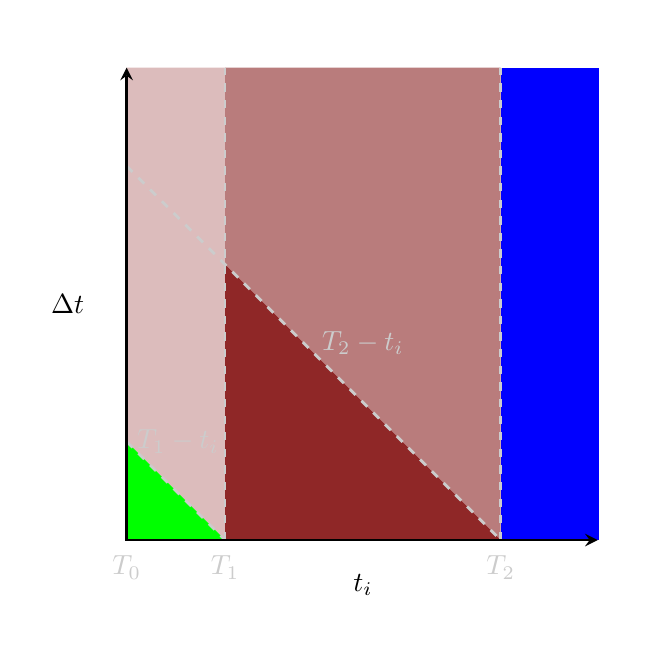
\begin{tikzpicture}[scale=1]
  \begin{scope}[shift={(0, 0)}]
    \draw[white] (-4.25, -4) rectangle (3.25, 3.5);
    
    \fill[light] (-3, 3) -- (-3, -1.75) -- (-1.75, -3) -- (-1.75, 3) -- cycle;
    
    \fill[mid] (-1.75, 3) -- (-1.75, 0.5) -- (+1.75, -3) -- (+1.75, 3) -- cycle;
    
    \fill[dark] (-1.75, -3) -- (-1.75, 0.5) -- (+1.75, -3) -- cycle;
    
    \fill[blue] (1.75, -3) -- (3, -3) -- (3, 3) -- (1.75, 3) -- cycle;
    
    \fill[green] (-3, -3) -- (-3, -1.75) -- (-1.75, -3) -- cycle;
    
    
    \node[gray80] at (-3, -3.35) { $T_{0}$ };
    
    \draw[gray80, line width=1, dashed] (-1.75, -3) -- (-1.75, 3);
    \node[gray80] at (-1.75, -3.35) { $T_{1}$ };
    
    \draw[gray80, line width=1, dashed] (+1.75, -3) -- (+1.75, 3);
    \node[gray80] at (+1.75, -3.35) { $T_{2}$ };
    
    %\draw[gray80, line width=1, dashed] (-3, -1.75) -- (3, -1.75);
    %\node[gray80] at (-3.35, -1.75) { $T_{1}$ };
    
    %\draw[gray80, line width=1, dashed] (-3, +1.75) -- (3, +1.75);
    %\node[gray80] at (-3.35, +1.75) { $T_{2}$ };
    
    \draw[gray80, line width=1, dashed] (-3, -1.75) -- (-1.75, -3);
    \node[gray80] at (0, -0.5) { $T_{2} - t_{i}$ };
    
    \draw[gray80, line width=1, dashed] (-3, +1.75) -- (+1.75, -3);
    \node[gray80] at (-2.35, -1.75) { $T_{1} - t_{i}$ };

    \draw [->, >=stealth, line width=1] (-3.0175, -3) -- +(6, 0);
    \draw [->, >=stealth, line width=1] (-3, -3) -- +(0, 6);
    \node at (0, -3.57) { $t_{i}$ };
    \node at (-3.75, 0) { $\Delta t$ };
  \end{scope}
   
\end{tikzpicture}

\end{document}  